% Options for packages loaded elsewhere
\PassOptionsToPackage{unicode}{hyperref}
\PassOptionsToPackage{hyphens}{url}
%
\documentclass[
  ignorenonframetext,
]{beamer}
\usepackage{pgfpages}
\setbeamertemplate{caption}[numbered]
\setbeamertemplate{caption label separator}{: }
\setbeamercolor{caption name}{fg=normal text.fg}
\beamertemplatenavigationsymbolsempty
% Prevent slide breaks in the middle of a paragraph
\widowpenalties 1 10000
\raggedbottom
\setbeamertemplate{part page}{
  \centering
  \begin{beamercolorbox}[sep=16pt,center]{part title}
    \usebeamerfont{part title}\insertpart\par
  \end{beamercolorbox}
}
\setbeamertemplate{section page}{
  \centering
  \begin{beamercolorbox}[sep=12pt,center]{part title}
    \usebeamerfont{section title}\insertsection\par
  \end{beamercolorbox}
}
\setbeamertemplate{subsection page}{
  \centering
  \begin{beamercolorbox}[sep=8pt,center]{part title}
    \usebeamerfont{subsection title}\insertsubsection\par
  \end{beamercolorbox}
}
\AtBeginPart{
  \frame{\partpage}
}
\AtBeginSection{
  \ifbibliography
  \else
    \frame{\sectionpage}
  \fi
}
\AtBeginSubsection{
  \frame{\subsectionpage}
}
\usepackage{amsmath,amssymb}
\usepackage{lmodern}
\usepackage{iftex}
\ifPDFTeX
  \usepackage[T1]{fontenc}
  \usepackage[utf8]{inputenc}
  \usepackage{textcomp} % provide euro and other symbols
\else % if luatex or xetex
  \usepackage{unicode-math}
  \defaultfontfeatures{Scale=MatchLowercase}
  \defaultfontfeatures[\rmfamily]{Ligatures=TeX,Scale=1}
\fi
\usetheme[]{Berkeley}
\usecolortheme{whale}
\usefonttheme{structurebold}
% Use upquote if available, for straight quotes in verbatim environments
\IfFileExists{upquote.sty}{\usepackage{upquote}}{}
\IfFileExists{microtype.sty}{% use microtype if available
  \usepackage[]{microtype}
  \UseMicrotypeSet[protrusion]{basicmath} % disable protrusion for tt fonts
}{}
\makeatletter
\@ifundefined{KOMAClassName}{% if non-KOMA class
  \IfFileExists{parskip.sty}{%
    \usepackage{parskip}
  }{% else
    \setlength{\parindent}{0pt}
    \setlength{\parskip}{6pt plus 2pt minus 1pt}}
}{% if KOMA class
  \KOMAoptions{parskip=half}}
\makeatother
\usepackage{xcolor}
\newif\ifbibliography
\usepackage{longtable,booktabs,array}
\usepackage{calc} % for calculating minipage widths
\usepackage{caption}
% Make caption package work with longtable
\makeatletter
\def\fnum@table{\tablename~\thetable}
\makeatother
\usepackage{graphicx}
\makeatletter
\def\maxwidth{\ifdim\Gin@nat@width>\linewidth\linewidth\else\Gin@nat@width\fi}
\def\maxheight{\ifdim\Gin@nat@height>\textheight\textheight\else\Gin@nat@height\fi}
\makeatother
% Scale images if necessary, so that they will not overflow the page
% margins by default, and it is still possible to overwrite the defaults
% using explicit options in \includegraphics[width, height, ...]{}
\setkeys{Gin}{width=\maxwidth,height=\maxheight,keepaspectratio}
% Set default figure placement to htbp
\makeatletter
\def\fps@figure{htbp}
\makeatother
\setlength{\emergencystretch}{3em} % prevent overfull lines
\providecommand{\tightlist}{%
  \setlength{\itemsep}{0pt}\setlength{\parskip}{0pt}}
\setcounter{secnumdepth}{-\maxdimen} % remove section numbering
\AtBeginSubsection{}
\AtBeginSection{}
\definecolor{unbc}{HTML}{035642}
\setbeamercolor{structure}{fg=unbc}
\setbeamertemplate{navigation symbols}{}
\setbeamertemplate{footline}[page number]
\ifLuaTeX
  \usepackage{selnolig}  % disable illegal ligatures
\fi
\IfFileExists{bookmark.sty}{\usepackage{bookmark}}{\usepackage{hyperref}}
\IfFileExists{xurl.sty}{\usepackage{xurl}}{} % add URL line breaks if available
\urlstyle{same} % disable monospaced font for URLs
\hypersetup{
  pdftitle={Research Proposal},
  pdfauthor={Akihiko Mori, MA NRES UNBC},
  hidelinks,
  pdfcreator={LaTeX via pandoc}}

\title{Research Proposal}
\subtitle{Measuring Food Waste in Prince George Restaurant: Volume,
Model, and Effects}
\author{Akihiko Mori, MA NRES UNBC}
\date{January 01, 2023}

\begin{document}
\frame{\titlepage}

\begin{frame}[allowframebreaks]
  \tableofcontents[hideallsubsections]
\end{frame}
\hypertarget{introduction}{%
\section{Introduction}\label{introduction}}

\begin{frame}{Introduction}
\protect\hypertarget{introduction-1}{}
\begin{itemize}
\tightlist
\item
  One-third of food is lost or wasted around the world{[}1{]}.
\end{itemize}

\begin{itemize}
\tightlist
\item
  Around 1.3 billion tons of FWL is generated annually, and the rate is
  projected to grow by 44\% per year by 2025{[}2{]}.
\item
  Canada creates about 35 million tons and the largest waste generator
  per capita in western countries in 2016{[}3{]}.
\end{itemize}

\begin{itemize}
\tightlist
\item
  In BC, 40\% of the waste to landfills is organic waste, the majority
  is produced from domestic waste{[}4{]}.
\end{itemize}

\begin{itemize}
\tightlist
\item
  Limited number of studies have been conducted on the food supply side
\end{itemize}
\end{frame}

\begin{frame}{Introduction}
\protect\hypertarget{introduction-2}{}
\begin{block}{Research Questions}
\protect\hypertarget{research-questions}{}
\begin{itemize}
\tightlist
\item
  What is the average volume of food that is wasted during processing
  and consumption in restaurants?
\item
  What is the extent of food wastage in Japanese restaurants in Prince
  George?
\item
  What are the main factors contributing to food loss and waste?
\item
  To what extent is a social or environmental impact from food loss
  waste generated by a single restaurant?
\item
  What approaches are Japanese restaurant operators taking to reduce
  food waste generation?
\end{itemize}
\end{block}
\end{frame}

\hypertarget{literature-review}{%
\section{Literature Review}\label{literature-review}}

\begin{frame}{Literature Review}
\protect\hypertarget{literature-review-1}{}
\begin{block}{Definition of FLW}
\protect\hypertarget{definition-of-flw}{}
\begin{itemize}
\tightlist
\item
  No universally accepted definitions of FLW
\end{itemize}

\begin{longtable}[]{@{}ll@{}}
\toprule()
Organizations & Definition \\
\midrule()
\endhead
Food Loss by FAO & harvest/slaughter/catch \\
Food Waste by FAO & retail/ consumption \\
Food Waste by EU & Food removed from FSC \\
Food Loss by US & unused product from agri \\
Food Waste by US & Subcomponent of FL \\
\bottomrule()
\end{longtable}
\end{block}
\end{frame}

\begin{frame}{Literature Review}
\protect\hypertarget{literature-review-2}{}
\begin{block}{Five Measurements of FLW}
\protect\hypertarget{five-measurements-of-flw}{}
\begin{longtable}[]{@{}ll@{}}
\toprule()
Method & Note \\
\midrule()
\endhead
1.Self-report & individuals report FLW \\
& low cost but high dropouts \\
2.Survey & collect FLW by interview or questionnaire \\
& cost-effective but not accurate \\
3.Composition & sample and analysis at lab \\
& need special knowledge and equipment \\
4.Mass balance & material flow analysis \\
& limitation in waste factor assumptions \\
5.Direct weight & directly measure FLW \\
& most accurate but high cost \\
\bottomrule()
\end{longtable}
\end{block}
\end{frame}

\begin{frame}{Literature Review}
\protect\hypertarget{literature-review-3}{}
\begin{block}{Statistic Model}
\protect\hypertarget{statistic-model}{}
\begin{itemize}
\item
  \textbf{Multiple Linear Regression}
\item
  Ad: Simple and interpretable
\item
  Disad: Not suitable to time series
\item
  Disad: Stationary and Spurious
\item
  \textbf{Bayesian Modelling}
\item
  Ad: Flexible and adaptable to time series data
\item
  Disad: No appropriate result in some cases
\end{itemize}
\end{block}
\end{frame}

\begin{frame}{Literature Review}
\protect\hypertarget{literature-review-4}{}
\begin{block}{Effects of Food Loss and Waste}
\protect\hypertarget{effects-of-food-loss-and-waste}{}
\begin{itemize}
\tightlist
\item
  \textbf{Economic Loss}:
\item
  labour, material resources, time, and energy
\item
  \textbf{Environmental Impacts}:
\item
  water scarcity, soil erosion, and GHG
\end{itemize}
\end{block}
\end{frame}

\begin{frame}{Literature Review}
\protect\hypertarget{literature-review-5}{}
\begin{block}{Hypotheses}
\protect\hypertarget{hypotheses}{}
\begin{itemize}
\tightlist
\item
  Bullet 1
\item
  Bullet 2
\item
  Bullet 3
\end{itemize}
\end{block}
\end{frame}

\hypertarget{methods}{%
\section{Methods}\label{methods}}

\begin{frame}{Methods}
\protect\hypertarget{methods-1}{}
\begin{block}{Study Area}
\protect\hypertarget{study-area}{}
\begin{itemize}
\tightlist
\item
  Japanese restaurant in Prince George
\item
  open for lunch and dinner for three hours each, six days of a week
\end{itemize}
\end{block}
\end{frame}

\begin{frame}{Methods}
\protect\hypertarget{methods-2}{}
\begin{block}{Sample Collection}
\protect\hypertarget{sample-collection}{}
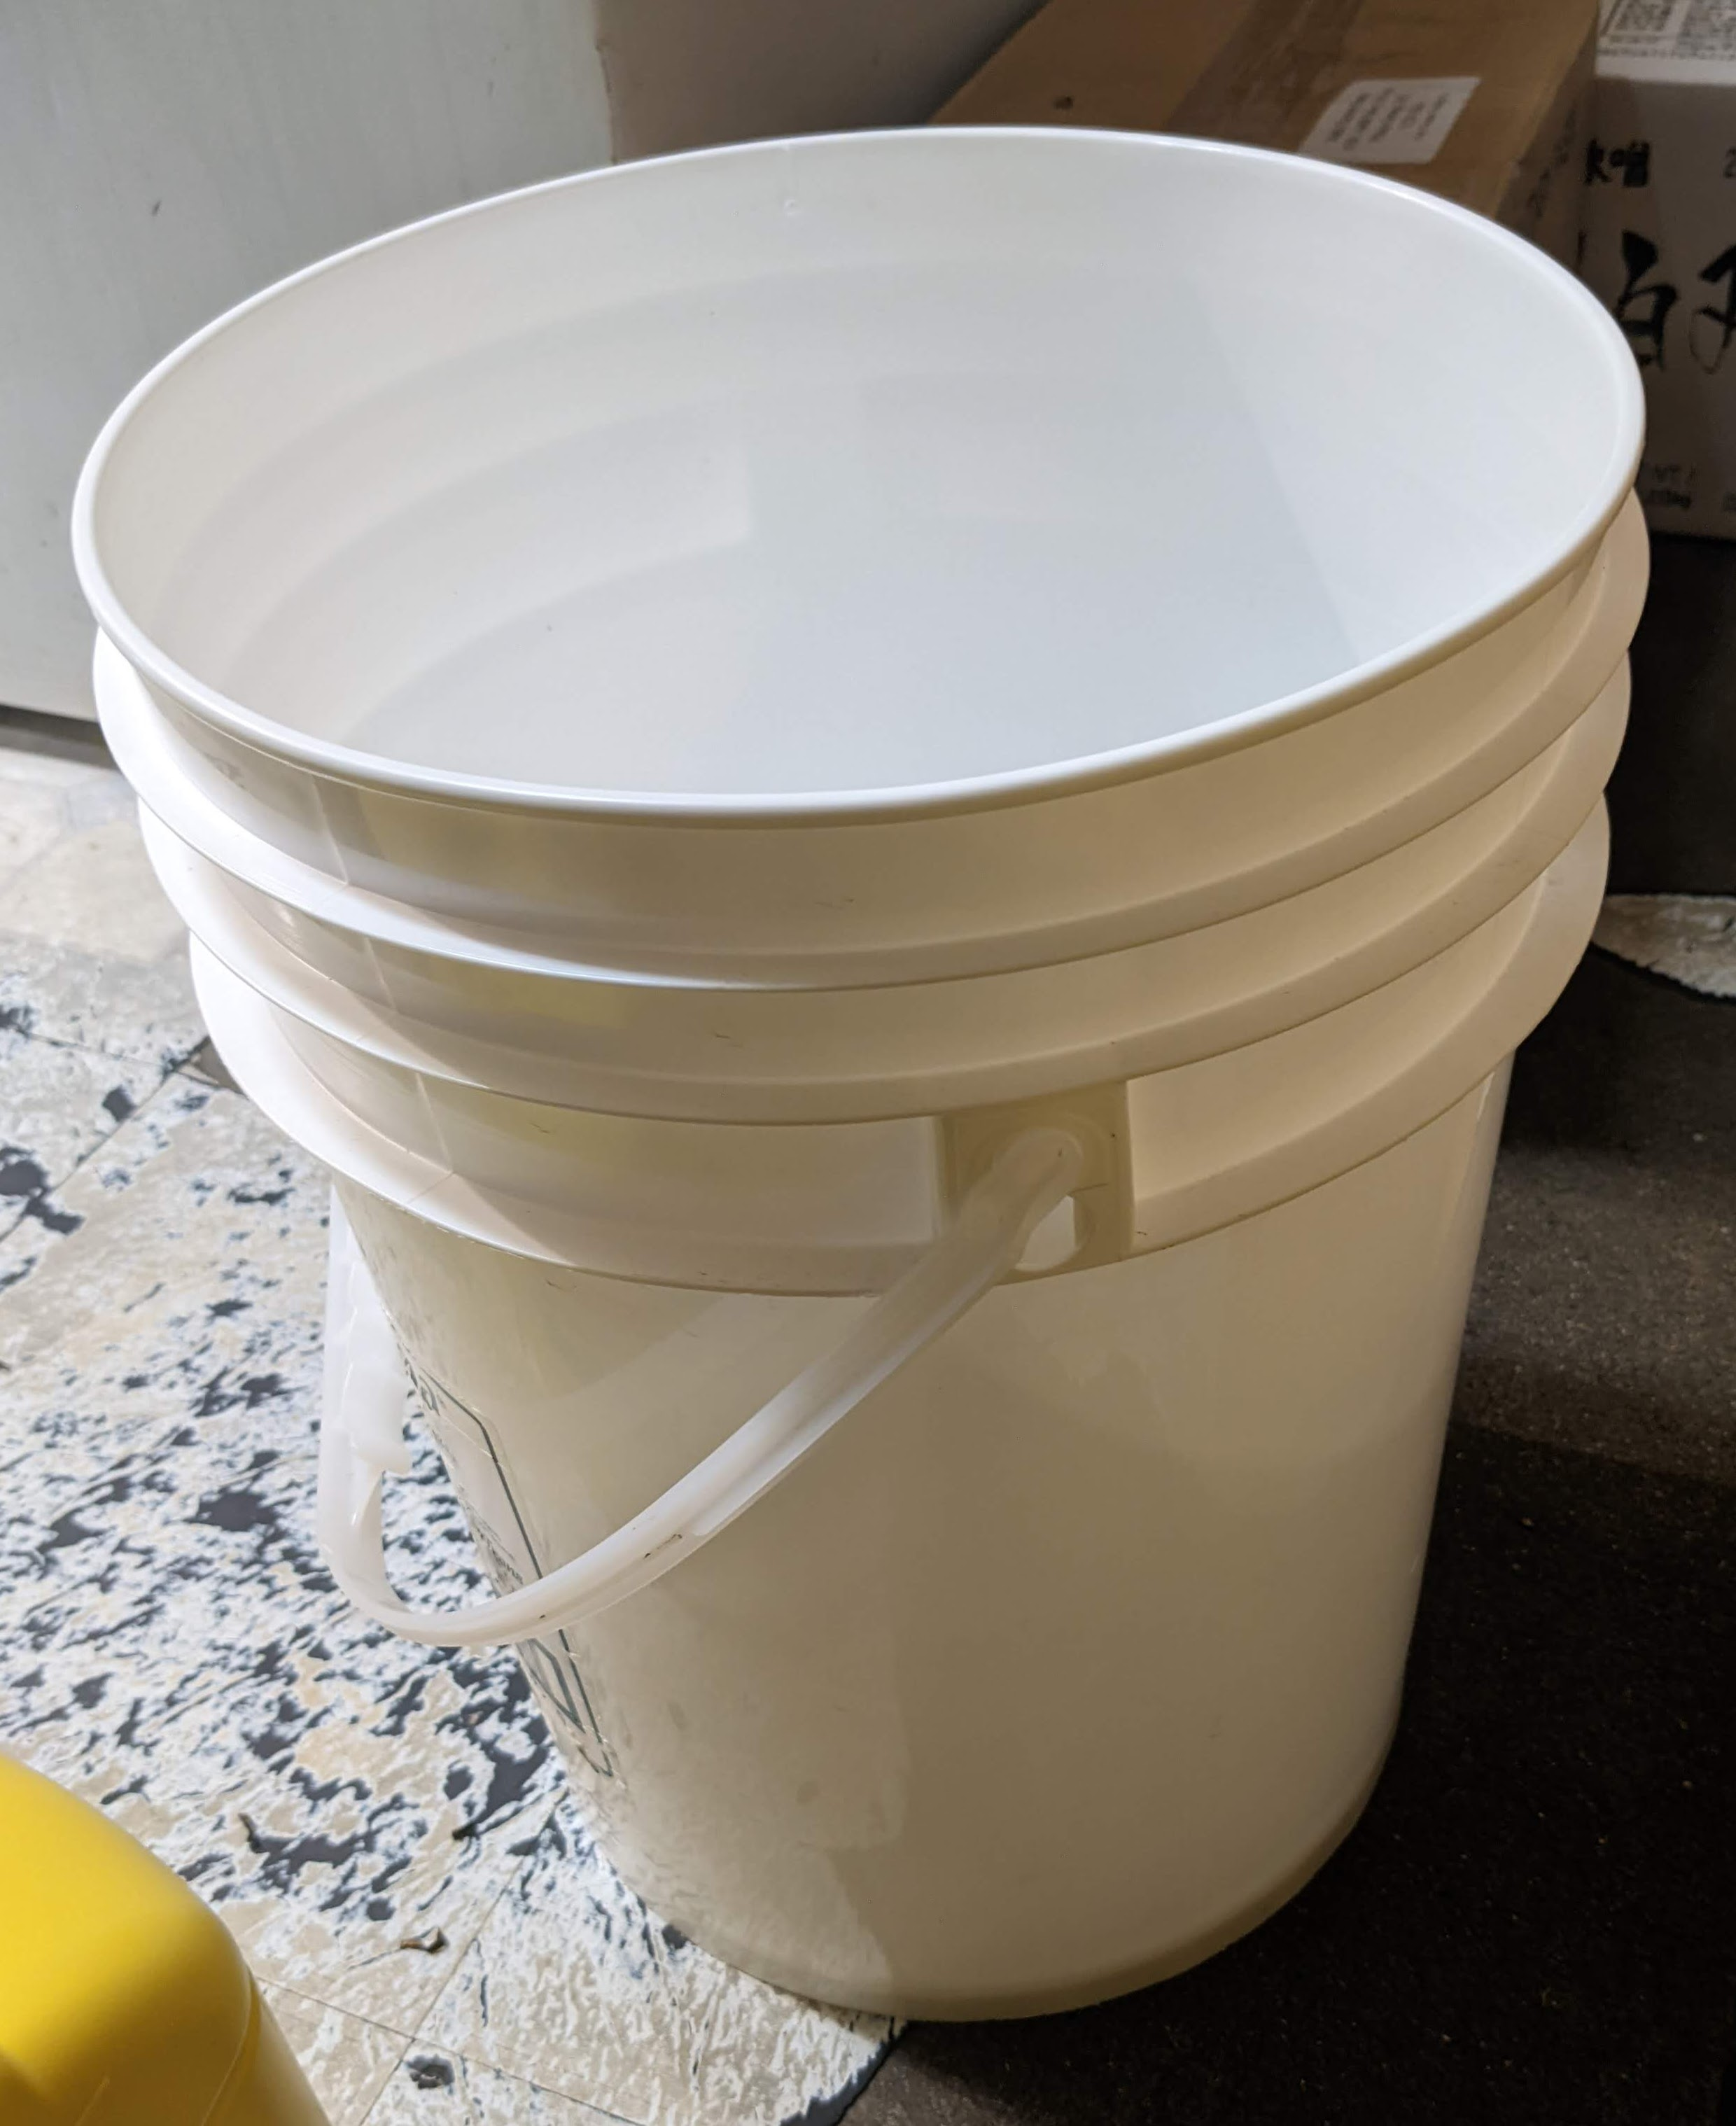
\includegraphics[width=0.4\textwidth,height=\textheight]{busket.jpg}
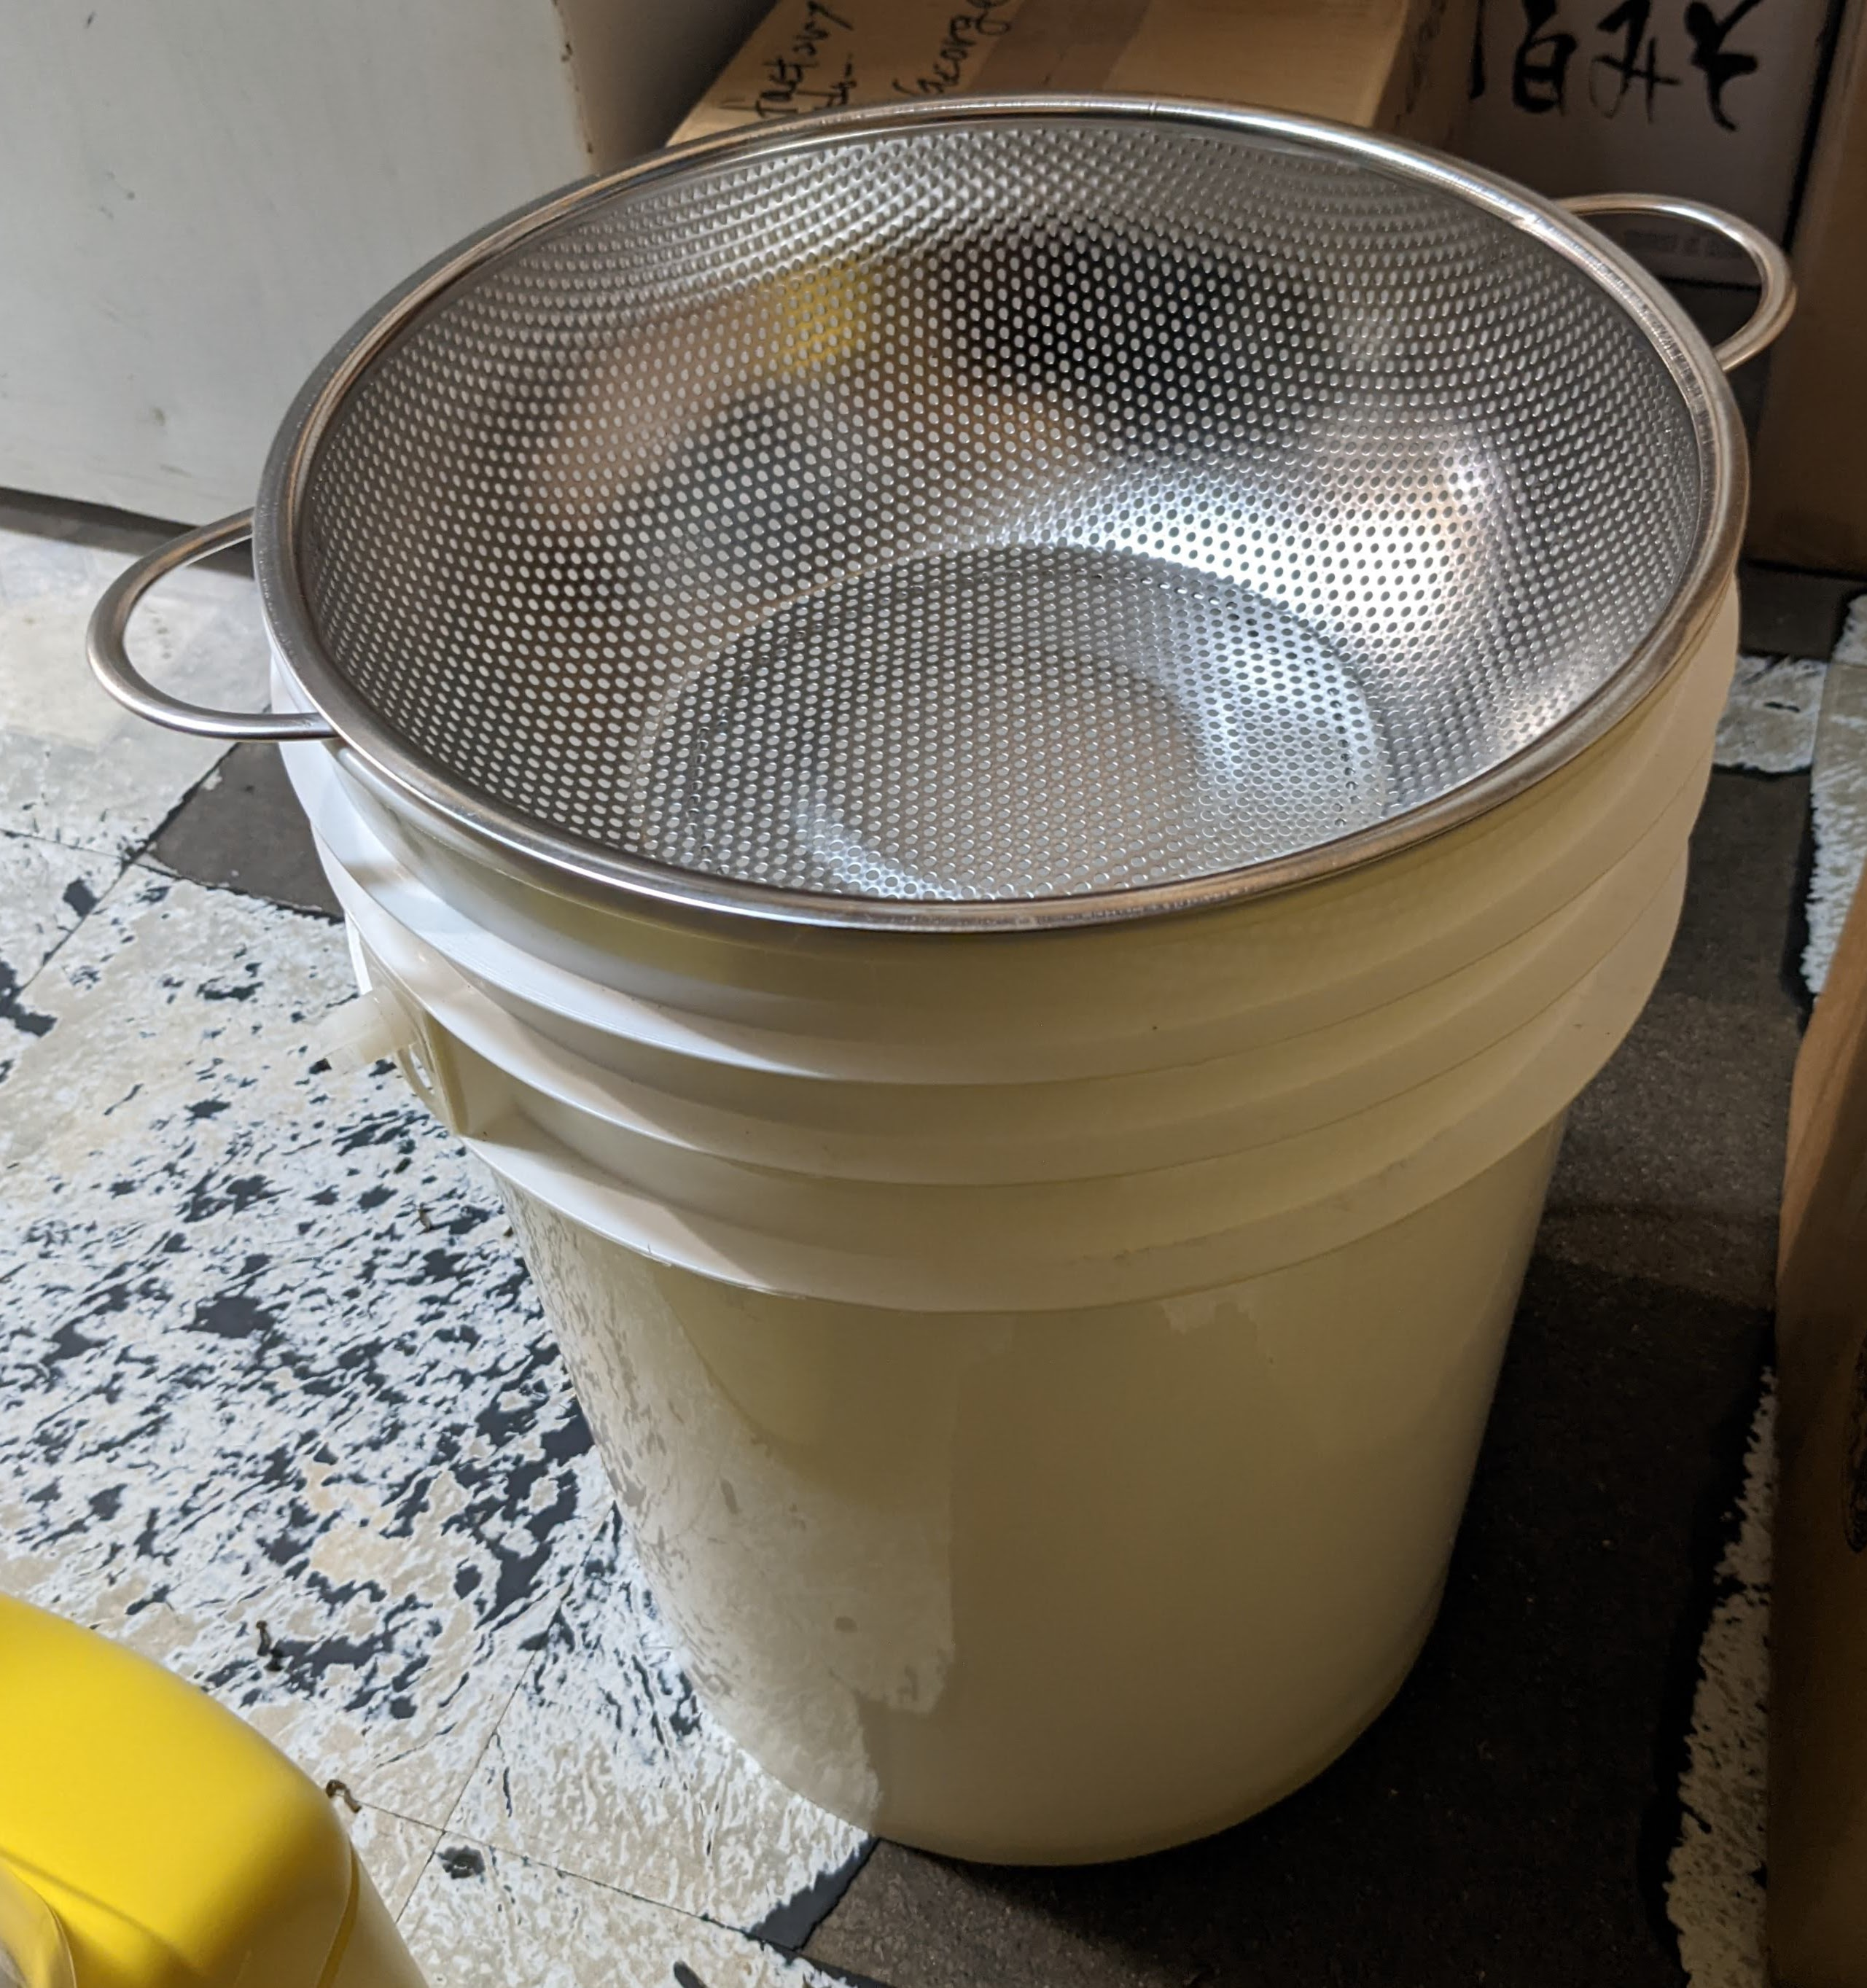
\includegraphics[width=0.45\textwidth,height=\textheight]{busketStrainer.jpg}
\end{block}
\end{frame}

\begin{frame}{Methods}
\protect\hypertarget{methods-3}{}
\begin{block}{Sample Size}
\protect\hypertarget{sample-size}{}
\begin{itemize}
\tightlist
\item
  By Power analysis, 95\% CI and 10\% margin of error with most
  conservative estimate says 97 samples{[}{]}
\item
  one in ten rule (rule-of-thumb) suggests 100 observations with 10
  predictors{[}{]}
\item
  Green's rule states 130 samples with 10 predictors{[}{]}
\end{itemize}
\end{block}
\end{frame}

\begin{frame}{Methods}
\protect\hypertarget{methods-4}{}
\begin{block}{Variables}
\protect\hypertarget{variables}{}
\begin{itemize}
\tightlist
\item
  Bullet 1
\item
  Bullet 2
\item
  Bullet 3
\end{itemize}
\end{block}
\end{frame}

\begin{frame}{Methods}
\protect\hypertarget{methods-5}{}
\begin{block}{Model}
\protect\hypertarget{model}{}
\begin{itemize}
\tightlist
\item
  Bullet 1
\item
  Bullet 2
\item
  Bullet 3
\end{itemize}
\end{block}
\end{frame}

\hypertarget{expected-results}{%
\section{Expected Results}\label{expected-results}}

\begin{frame}{Expected Results}
\protect\hypertarget{expected-results-1}{}
\begin{block}{Expected Results}
\protect\hypertarget{expected-results-2}{}
\end{block}
\end{frame}

\begin{frame}{Expected Results}
\protect\hypertarget{expected-results-3}{}
\begin{block}{Current Progress}
\protect\hypertarget{current-progress}{}
\begin{itemize}
\tightlist
\item
  From Sept.~16, four months.
\item
  Collected over 100 samples.
\item
\item
  Bullet 3
\end{itemize}
\end{block}
\end{frame}

\hypertarget{references}{%
\section{References}\label{references}}

\end{document}
